\documentclass[./\jobname.tex]{subfiles}
\begin{document}
\section{Theoretical Notes}
This chapter deals with a few theoretical notes. At first, the universal approximation theorem for the \gls{gsk} is shown. Further, the multimodality of the fitness function is proven. Thereby, a symmetry is observed that could lead to the design of better variation operators.  

\subsection{Universial Approximation Theorem}
\label{chap:gsin_approximation_theorem}

The Gauss kernel is able to approximate all functions that are part of the Lebesgue space $f(\mathbf{x}) \in L^1(\mathbb{R}^n)$ arbitrarily close. This has been proven by various works (\cite{park_universal_1991}, \cite{hangelbroek_nonlinear_2010}). In particular, \cite{park_universal_1991} extends the universal approximation theorem to other kernels. The following paragraphs show that the \gls{gsk} fulfils the posed conditions and thus can benefit from the approximation theorem. 

The Gauss-Sine kernel, as defined in equation \eqref{eq:gsin_kernel_theoretical_notes}, is a multiplication of the Gauss kernel with a sine function. Its main purpose is described in the experiment \mbox{chapter \ref{chap:experimet_3}}. 

\begin{equation}
\label{eq:gsin_kernel_theoretical_notes}
gsk(\mathbf{x}) = \omega e^{-\gamma ||\mathbf{x} - \mathbf{c}||^2} sin(f ||\mathbf{x} - \mathbf{c}||^2 - \varphi)
\end{equation}

To prove that the universal approximation theorem is also applicable to the \gls{gsk}, it must comply with the conditions placed by \cite{park_universal_1991}. At first, a kernel, in this case the $gsk(\mathbf{x})$, must be continuous and bounded. This already restricts $\gamma > 0$. However, \cite{chaquet_using_2019} found that not placing any limits on the parameters results in a better performance. Thus, this constraint is not implemented in the current version of the algorithm. Secondly, the integral over the whole domain of the kernel $K(\mathbf{x})$ must not be $0$. Thus, it needs to be shown that 

\begin{equation}
\int_{\mathbf{x} = -\mathbf{\infty}}^{\infty} gsk(\mathbf{x}) \text{ } d\mathbf{x} \neq 0
\end{equation} 

Intuitively, the next restriction on $\omega \neq 0$ is found. 

To simplify the following calculations, the \gls{gsk} is rewritten into polar coordinates. Further, the offsets by $c_0$ and $c_1$ are accounted for by an appropriate coordinate transformation. This results in 

\begin{equation}
\lim_{t \to \infty} \int_{r=0}^{t} \int_{\theta = 0}^{2 \pi} e^{-\gamma(r^2)} sin(f r^2 - \varphi) r \text{ } dr \text{ } d\theta
\end{equation}

Since the kernel is radial symmetric and thus has no dependency on $\theta$, the respective integral can be solved immediately which results in a multiplicative factor of $2 \pi$. The integral can be further simplified by substituting $r^2 = u$.
The resulting expression can be solved with ``integration by part'' $\int f(u) \frac{g(u)}{du} = f(u) g(u) - \int g(u) \frac{f(u)}{du}$. The formula has to be applied twice. 

\begin{equation}
\begin{split}
& 2 \pi \lim_{t \to \infty} \int_{r=0}^{t} e^{-\gamma(r^2)} sin(f r^2 - \varphi) r \text{ } dr  \\
= & \pi \lim_{t \to \infty} \int_{u=0}^{t} \underbrace{e^{-\gamma u }}_{\frac{g(u)}{du}} \underbrace{sin(f u - \varphi)}_{f(u)} \text{ } du \\
= - \frac{sin(fu - \varphi) e^{-\gamma u}}{\gamma} +\frac{f}{\gamma} & \left[ -cos(fu -\varphi) \frac{e^{-\gamma u}}{\gamma} -\frac{f}{\gamma} \int e^{-\gamma u} sin(fu -\varphi) du \right] \\
\end{split}
\end{equation}

The same integral is retrieved. Thus, the equation can be rearranged and solved for the integral. Considering the constant factors and the integral limits gives 

\begin{equation}
\lim_{t \to \infty} \frac{\pi e^{-\gamma r^2}(- \gamma sin(f r^2 - \varphi) - f cos(f r^2 - \varphi))}{ \gamma^2 + f^2} + C \text{ } \Bigg|_{r=0}^{t}.
\end{equation}

To resolve the limit of the function towards $\infty$, the function value must be bounded. Therefore, $\gamma$ must be positive, which is already required. Finally, this results in 

\begin{equation}
	\frac{-\pi (\gamma sin(\varphi) + f cos(\varphi))}{\gamma^2 + f^2} \neq 0.
\end{equation}

This places more constraints on the parameter of the \gls{gsk} as seen in the equation \eqref{eq:gsk_param_restrictions} below. 

\begin{equation}
\label{eq:gsk_param_restrictions}
	\begin{split}
	\gamma & > 0 \\
	\omega & \neq 0 \\
	\gamma & sin(\varphi) + f cos(\varphi) \neq 0 \\
	\end{split}
\end{equation}

These restrictions on the parameters could be enforced during the optimisation process. They could further be used to limit the search dimension. Thus, other optimisation algorithms, that are good at handling constraints must be used. 

\subsection{Multimodality and Symmetry}
\label{chap:multimodality_and_symmetry}

The optimisation algorithm tries to find the best approximation of $N$ kernels to the solution of a differential equation. Assume, that a kernel $K$ is fully defined by a vector of parameters $\mathbf{p}$. The best fit is defined as 

\begin{equation}
\mathbf{\hat{p}_{apx}} = \left[\underbrace{\left[ \mathbf{\hat{p}}_{K_0} \right] }_{\text{kernel 0}}, \cdots \underbrace{\left[ \mathbf{\hat{p}}_{K_i} \right] }_{\text{kernel i}}, \cdots \underbrace{\left[ \mathbf{\hat{p}}_{K_N} \right]}_{\text{kernel N}} \right]^T
\end{equation}

where the parameters $\mathbf{\hat{p}}$ of every kernel are chosen optimally. The optimal kernel functions $K(\mathbf{\hat{p}}_{K_i}, \mathbf{x})$ are summed up to form the optimal approximation $\hat{u}_{apx}(\mathbf{x})$. 

\begin{equation}
\label{eq:uapx_kernel_sum}
\hat{u}_{apx}(\mathbf{x}) = \sum_{i=0}^{N} K(\mathbf{\hat{p}}_{K_i}, \mathbf{x})
\end{equation}

Since the order of the summation is irrelevant, any kernel-wise permutation describes an optimal solution $\mathbf{\hat{p}_{apx}}$. Thus, the fitness function $F(u_{apx}(\mathbf{x}))$ has at least $N!$ number of local optima and all of them share the same function value. 

Further, a symmetry in the location of the optima is observed. All optima lay on the surface of the hypersphere that is centred at the origin and has a radius of $r = || \mathbf{\hat{p}_{apx}} ||$. 

The following 3D plot in figure \ref{fig:optima_distribution} shows an exemplary distribution of optima on the fitness function. For the sake of simplicity, a kernel now consists of only one parameter. As an example, the vector $\mathbf{\hat{p}_{apx}} = \left[ 2, 1, -1 \right]^T$ describes an optimal solution that consists of 3 kernels. Any permutation of these three coordinates is itself a perfect fit. 

\begin{figure}[H]
	\centering
	\noindent\adjustbox{max width=0.7\linewidth}{
		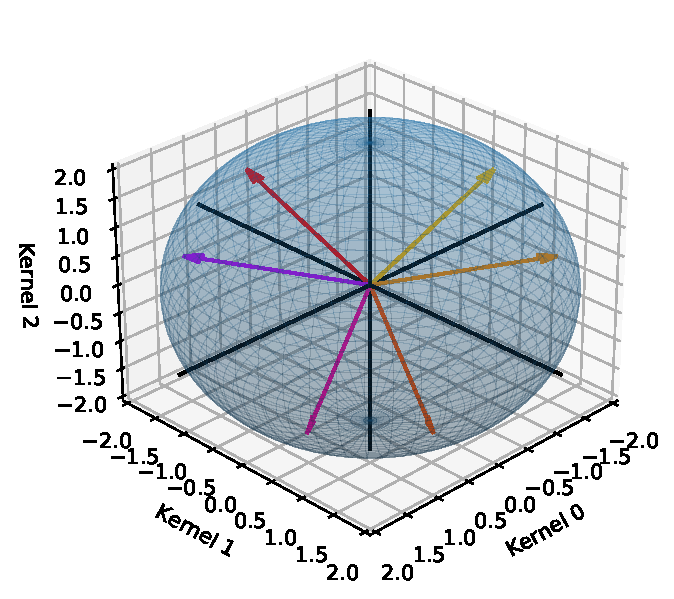
\includegraphics[width=\textwidth]{../img/pdf/symmetry.pdf}
	}
	\unterschrift{Distribution of exemplary optima on the fitness function in 3D space.}{}{}
	\label{fig:optima_distribution}
\end{figure}

This symmetry is independent of the kernel type. Large parts of the fitness function, such as the weighting and penalty factors or the number of collocation points, have no influence on the actual radial arrangement of the optima. The symmetry is a fundamental property of the sum of \gls{rbf}. Thus, it could even be applied in other fields that use this kind of representation. One of these could be non-linear function approximation. 

Obviously, the order of summation is not only true for the optimum, but also for every other point in between. Thus, the entire fitness function exhibits this radial symmetry. More work investigating the structure of the fitness function must be done. With more knowledge about the features of this function, it might be possible to design algorithms specifically to that problem. 

\end{document}